\documentclass[12pt,a4paper]{article}

\usepackage[utf8]{inputenc}
\usepackage[spanish]{babel}
\usepackage{graphicx}
\usepackage{geometry}
\geometry{a4paper, margin=2.5cm}
\usepackage{xcolor}
\usepackage{listings}
\usepackage{booktabs}
\usepackage{amsmath}
\usepackage{subcaption}
\usepackage{float}
\usepackage[colorlinks=true, linkcolor=blue, urlcolor=blue]{hyperref}

\definecolor{codegreen}{rgb}{0,0.6,0}
\definecolor{codegray}{rgb}{0.5,0.5,0.5}
\definecolor{codepurple}{rgb}{0.58,0,0.82}
\definecolor{backcolour}{rgb}{0.95,0.95,0.92}

\lstdefinestyle{mystyle}{
    backgroundcolor=\color{backcolour},   
    commentstyle=\color{codegreen},
    keywordstyle=\color{magenta},
    numberstyle=\tiny\color{codegray},
    stringstyle=\color{codepurple},
    basicstyle=\ttfamily\footnotesize,
    breakatwhitespace=false,         
    breaklines=true,                 
    captionpos=b,                    
    keepspaces=true,                 
    numbers=left,                    
    numbersep=5pt,                  
    showspaces=false,                
    showstringspaces=false,
    showtabs=false,                  
    tabsize=2
}
\lstset{style=mystyle}

\title{\Huge\textbf{PROYECTO ESP32} \\ \Large On/Off por Teclado (Keyboard) \\ \vspace{0.5cm} \normalsize \textit{Control de un LED mediante comandos enviados por el Monitor Serial}}
\author{Msc. Néstor Fabio Montoya Palacios}
\date{2026 \\ \vspace{0.2cm} \small Plataforma: ESP32 Dev Module}

\begin{document}

\maketitle
\tableofcontents
\newpage

% ══════════════════════════════════════════════════════════════
\section{Introducción}
% ══════════════════════════════════════════════════════════════

Este documento describe de manera detallada el proyecto ``On/Off Keyboard'', un circuito interactivo que permite al usuario controlar el encendido y apagado de un LED conectado al ESP32 mediante comandos de teclado enviados a través del Monitor Serial del Arduino IDE.

A diferencia del proyecto ``On/Off Repetitivo'' ---donde el LED parpadea automáticamente---, en este proyecto el usuario tiene el control total: al presionar la tecla \texttt{a} el LED se enciende, y al presionar la tecla \texttt{b} el LED se apaga. Esto introduce conceptos fundamentales de \textbf{comunicación serial}, \textbf{lectura de datos de entrada} y \textbf{toma de decisiones condicionales} en la programación de microcontroladores.

El ESP32 es un microcontrolador de bajo costo y alto rendimiento desarrollado por Espressif Systems. Cuenta con conectividad Wi-Fi y Bluetooth integrada, lo que lo convierte en una plataforma ideal tanto para proyectos educativos como para aplicaciones IoT profesionales.

Este proyecto sirve como segundo paso en el aprendizaje de Arduino, consolidando los conceptos de GPIO y comunicación serial mientras introduce la interacción usuario-microcontrolador en tiempo real.

% ══════════════════════════════════════════════════════════════
\section{Objetivo del Proyecto}
% ══════════════════════════════════════════════════════════════

Implementar un sistema de control manual de un LED utilizando el microcontrolador ESP32, donde el usuario envía comandos desde el teclado del computador a través del Monitor Serial, demostrando el uso de:
\begin{itemize}
    \item Salidas digitales (GPIO) para controlar un actuador (LED).
    \item Comunicación serial bidireccional (lectura y escritura).
    \item Estructuras condicionales (\texttt{if / else if}) para la toma de decisiones.
    \item Lectura de caracteres individuales desde el buffer serial.
\end{itemize}

% ══════════════════════════════════════════════════════════════
\section{Materiales Necesarios}
% ══════════════════════════════════════════════════════════════

\begin{table}[h!]
\centering
\begin{tabular}{cll}
\toprule
\textbf{Cant.} & \textbf{Componente} & \textbf{Especificación} \\
\midrule
1 & ESP32 Dev Module & Microcontrolador con Wi-Fi/Bluetooth \\
1 & LED (5mm) & LED difuso, $V_f \approx 2V$, $I_f \approx 20mA$ \\
1 & Resistencia 220 $\Omega$ & 1/4W, tolerancia 5\% \\
1 & Protoboard & Placa de pruebas de 830 puntos \\
2 & Cables jumper & Macho-macho para conexiones \\
1 & Cable USB Micro-B & Para programación y alimentación \\
\bottomrule
\end{tabular}
\caption{Lista de materiales del proyecto On/Off Keyboard}
\end{table}

% ══════════════════════════════════════════════════════════════
\section{Esquema de Conexión}
% ══════════════════════════════════════════════════════════════

El siguiente esquema, realizado en Fritzing, muestra las conexiones físicas del circuito. El LED está conectado al pin D4 (GPIO4) del ESP32 a través de una resistencia limitadora de corriente de 220 $\Omega$. El cátodo del LED se conecta a la línea de tierra (GND) del ESP32.

\textbf{Nota:} El esquema de conexión es el mismo utilizado en el proyecto ``On/Off Repetitivo'', ya que el hardware es idéntico; la diferencia radica exclusivamente en el software (firmware) cargado en el ESP32.

\begin{figure}[H]
\centering
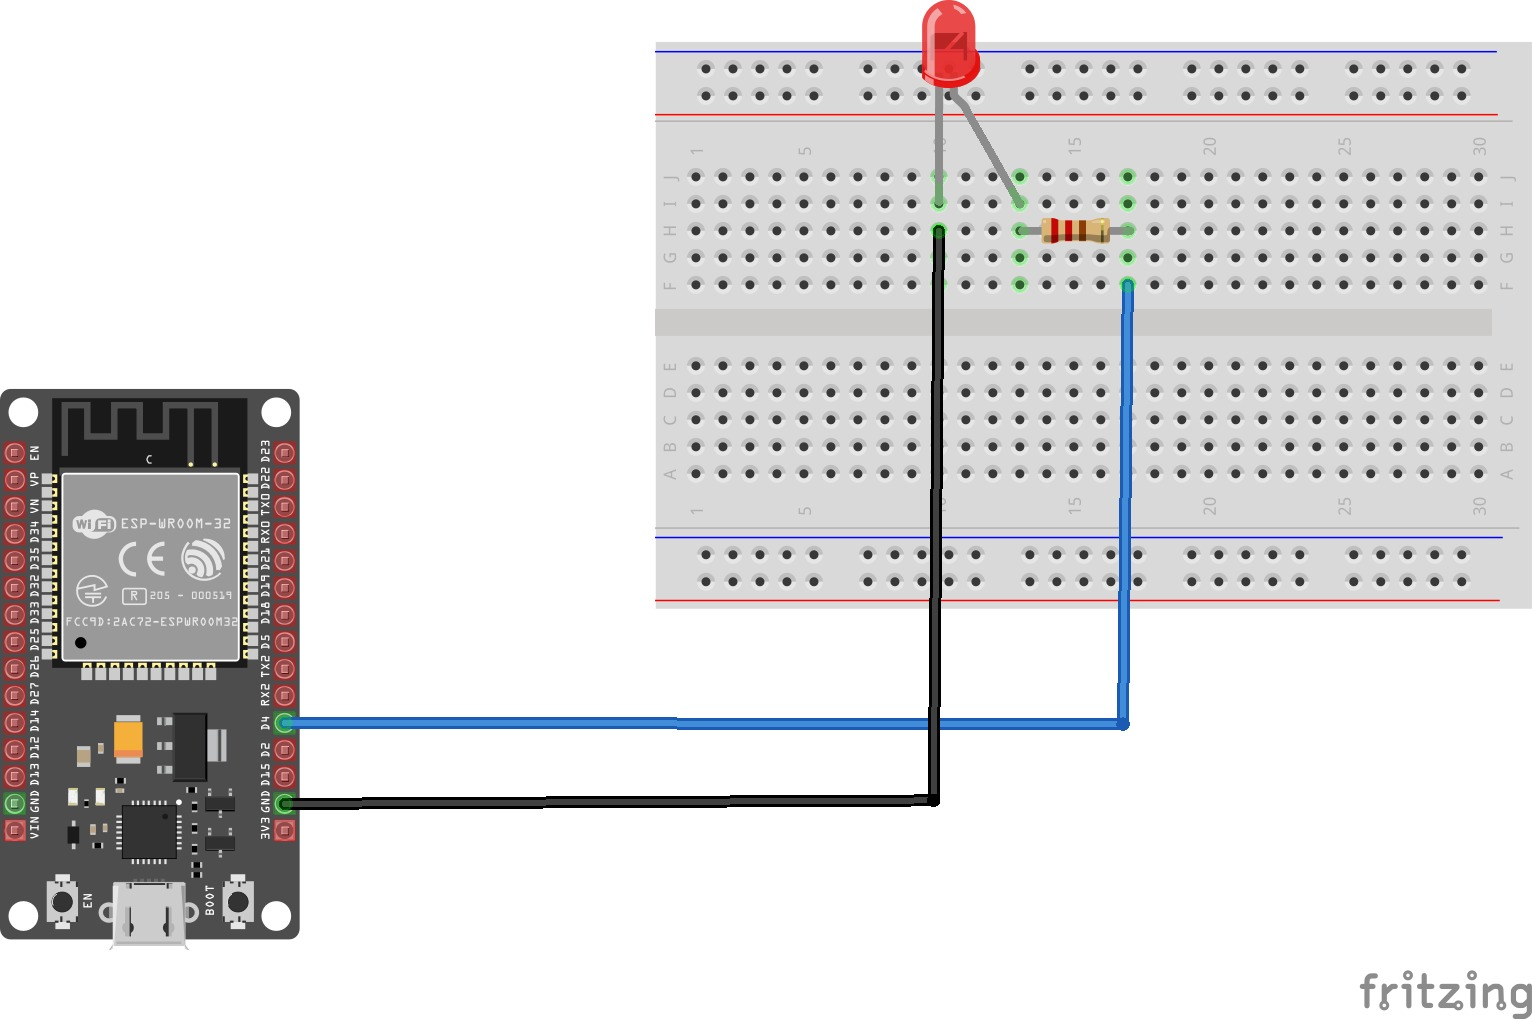
\includegraphics[width=0.85\textwidth]{../Esquemas/On_Off_Repetitivo_esq.jpeg}
\caption{Esquema de conexión del circuito On/Off Keyboard (Fritzing)}
\label{fig:esquema}
\end{figure}

\subsection{Descripción de las Conexiones}
\begin{enumerate}
    \item \textbf{Pin D4 (GPIO4)} del ESP32 se conecta al ánodo (+) del LED mediante un cable jumper (azul en el esquema).
    \item El \textbf{cátodo (--)} del LED se conecta a un extremo de la resistencia de 220 $\Omega$.
    \item El otro extremo de la resistencia se conecta al \textbf{bus de tierra (GND)} de la protoboard.
    \item El \textbf{pin GND} del ESP32 se conecta al bus de tierra de la protoboard con un cable negro.
\end{enumerate}

\subsection{Diagrama Esquemático del Circuito}
El circuito se puede representar de forma simplificada como:

\begin{center}
\texttt{ESP32 GPIO4} $\longrightarrow$ \texttt{LED (ánodo $\to$ cátodo)} $\longrightarrow$ \texttt{R = 220\,$\Omega$} $\longrightarrow$ \texttt{GND}
\end{center}

% ══════════════════════════════════════════════════════════════
\section{Código Fuente}
% ══════════════════════════════════════════════════════════════

A continuación se presenta el código completo del proyecto con explicación detallada de cada sección:

\subsection{Código Completo (On\_Off\_Keyboard.ino)}
\begin{lstlisting}[language=C++, title=On\_Off\_Keyboard.ino]
/*
 * ════════════════════════════════════════════════════
 *  Control de LED por teclado Serial - ESP32
 *  Tecla 'a' -> Enciende el LED
 *  Tecla 'b' -> Apaga el LED
 *  Autor : Msc. Nestor Fabio Montoya Palacios
 *  Fecha : 2026
 *  Board : ESP32 Dev Module
 * ════════════════════════════════════════════════════
 */

const int PIN_LED = 4;

void setup() {
  Serial.begin(115200);
  pinMode(PIN_LED, OUTPUT);
  digitalWrite(PIN_LED, LOW);

  Serial.println("Presiona 'a' para encender el LED");
  Serial.println("Presiona 'b' para apagar el LED");
}

void loop() {

  if (Serial.available() > 0) {

    char tecla = Serial.read();

    if (tecla == 'a' || tecla == 'A') {
      digitalWrite(PIN_LED, HIGH);
      Serial.println("LED ENCENDIDO");

    } else if (tecla == 'b' || tecla == 'B') {
      digitalWrite(PIN_LED, LOW);
      Serial.println("LED APAGADO");
    }
  }
}
\end{lstlisting}
\textit{Nota: Se han simplificado los caracteres decorativos del código original para garantizar la compatibilidad con el compilador de \LaTeX.}

% ══════════════════════════════════════════════════════════════
\subsection{Análisis del Código}
% ══════════════════════════════════════════════════════════════

\subsubsection*{Encabezado y Constantes}
El programa comienza con un bloque de comentarios que documenta el propósito, autor y plataforma. Luego se define una única constante:
\begin{itemize}
    \item \textbf{\texttt{PIN\_LED = 4}:} Define el pin GPIO\,4 como la salida digital que controlará el LED. Usar una constante permite cambiar fácilmente el pin sin modificar múltiples líneas de código.
\end{itemize}

\subsubsection*{Función \texttt{setup()}}
Esta función se ejecuta una sola vez al iniciar (o reiniciar) el ESP32. Realiza tres tareas fundamentales:

\begin{enumerate}
    \item \textbf{\texttt{Serial.begin(115200)}:} Inicializa la comunicación serial UART a una velocidad de 115200 baudios. Este valor debe coincidir con la configuración del Monitor Serial en el Arduino IDE para que la comunicación funcione correctamente.
    
    \item \textbf{\texttt{pinMode(PIN\_LED, OUTPUT)}:} Configura el pin GPIO4 como \textit{salida digital}, habilitándolo para enviar señales de voltaje alto (3.3V) o bajo (0V).
    
    \item \textbf{\texttt{digitalWrite(PIN\_LED, LOW)}:} Establece el estado inicial del LED como apagado (0V en el pin).
    
    \item \textbf{Mensajes de instrucciones:} Se imprimen dos líneas en el Monitor Serial indicando al usuario qué teclas debe presionar para controlar el LED. Esto proporciona una interfaz de usuario básica por consola.
\end{enumerate}

\subsubsection*{Función \texttt{loop()}}
Esta función se ejecuta en un ciclo infinito y contiene la lógica principal del programa. A diferencia del proyecto ``On/Off Repetitivo'' (que usa \texttt{delay()}), este programa utiliza un modelo \textbf{basado en eventos}: solo actúa cuando hay datos disponibles en el buffer serial.

\begin{enumerate}
    \item \textbf{\texttt{Serial.available() > 0}:} Verifica si hay datos pendientes en el buffer de recepción serial. Retorna el número de bytes disponibles para leer. Si no hay datos, el \texttt{loop()} simplemente se repite sin hacer nada, lo que mantiene al microcontrolador receptivo.
    
    \item \textbf{\texttt{Serial.read()}:} Lee y retorna el primer byte (carácter) disponible en el buffer serial, almacenándolo en la variable \texttt{tecla} de tipo \texttt{char}.
    
    \item \textbf{Estructura condicional:}
    \begin{itemize}
        \item Si \texttt{tecla == 'a'} o \texttt{tecla == 'A'}: Se enciende el LED (\texttt{HIGH}) y se confirma por serial.
        \item Si \texttt{tecla == 'b'} o \texttt{tecla == 'B'}: Se apaga el LED (\texttt{LOW}) y se confirma por serial.
        \item Cualquier otro carácter es simplemente ignorado.
    \end{itemize}
\end{enumerate}

La aceptación de mayúsculas y minúsculas (\texttt{'a'} y \texttt{'A'}) hace el programa más robusto y amigable para el usuario.

% ══════════════════════════════════════════════════════════════
\section{Principio de Funcionamiento}
% ══════════════════════════════════════════════════════════════

\subsection{Comunicación Serial (UART)}
El proyecto se basa en la comunicación \textbf{UART} (Universal Asynchronous Receiver-Transmitter) entre el ESP32 y el computador a través del cable USB. El flujo de datos es el siguiente:

\begin{enumerate}
    \item El usuario escribe un carácter en el campo de texto del Monitor Serial del Arduino IDE.
    \item Al presionar ``Enviar'' (o Enter), el carácter se transmite como un byte ASCII a través del cable USB.
    \item El chip USB-UART del ESP32 convierte la señal USB a señal UART y la deposita en el buffer de recepción serial.
    \item La función \texttt{Serial.available()} detecta que hay datos y \texttt{Serial.read()} lee el byte.
    \item El programa evalúa el carácter y actúa en consecuencia.
    \item La respuesta (\texttt{"LED ENCENDIDO"} o \texttt{"LED APAGADO"}) se envía de vuelta al computador por el mismo canal serial.
\end{enumerate}

\subsection{Control del GPIO}
Cuando el ESP32 escribe un valor \texttt{HIGH} en el pin GPIO4, este entrega aproximadamente 3.3V, lo cual permite que la corriente fluya a través del LED y la resistencia, encendiendo el LED. Al escribir \texttt{LOW}, el pin se pone a 0V y el LED se apaga.

\subsection{Cálculo de la Corriente}
La resistencia de 220 $\Omega$ cumple la función crítica de limitar la corriente que circula por el LED. Sin esta resistencia, la corriente excesiva dañaría el LED. El cálculo de la corriente es:

\begin{equation}
I = \frac{V_{gpio} - V_{led}}{R} = \frac{3.3\text{ V} - 2.0\text{ V}}{220\,\Omega} \approx 5.9\text{ mA}
\label{eq:corriente}
\end{equation}

Este valor está dentro del rango seguro de operación tanto para el LED (máx.\ 20\,mA) como para el pin del ESP32 (máx.\ 40\,mA por pin).

% ══════════════════════════════════════════════════════════════
\section{Comparación con el Proyecto On/Off Repetitivo}
% ══════════════════════════════════════════════════════════════

\begin{table}[H]
\centering
\begin{tabular}{lll}
\toprule
\textbf{Característica} & \textbf{On/Off Repetitivo} & \textbf{On/Off Keyboard} \\
\midrule
Tipo de control & Automático & Manual (usuario) \\
Uso de \texttt{delay()} & Sí (bloquea ejecución) & No \\
Comunicación serial & Solo escritura & Lectura y escritura \\
Interacción del usuario & Ninguna & Envía comandos por teclado \\
Modelo de ejecución & Secuencial con pausas & Basado en eventos \\
Circuito (hardware) & Idéntico & Idéntico \\
\bottomrule
\end{tabular}
\caption{Comparación entre los proyectos On/Off Repetitivo y On/Off Keyboard}
\end{table}

% ══════════════════════════════════════════════════════════════
\section{Fotografías del Montaje}
% ══════════════════════════════════════════════════════════════

Las siguientes imágenes muestran el proyecto montado y en funcionamiento:

\begin{figure}[H]
    \centering
    \begin{subfigure}[b]{0.48\textwidth}
        \centering
        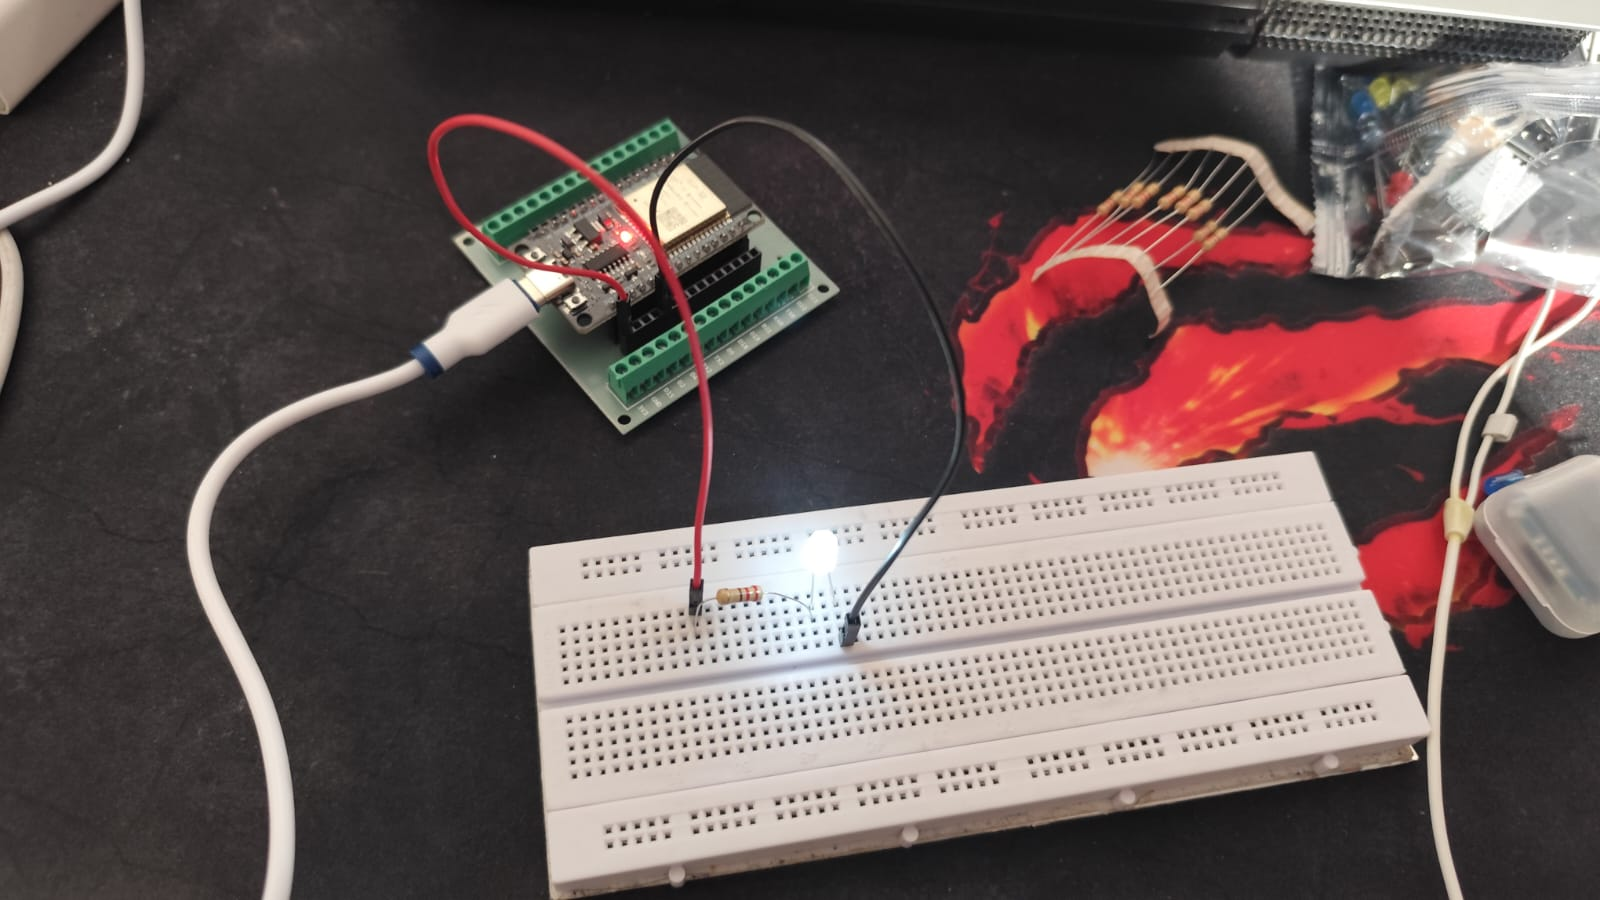
\includegraphics[width=\textwidth]{../Imagenes/On_Off_keyboard_imgs/On_Off_keyboard_img2.jpeg}
        \caption{Circuito con LED encendido}
        \label{fig:led_on}
    \end{subfigure}
    \hfill
    \begin{subfigure}[b]{0.48\textwidth}
        \centering
        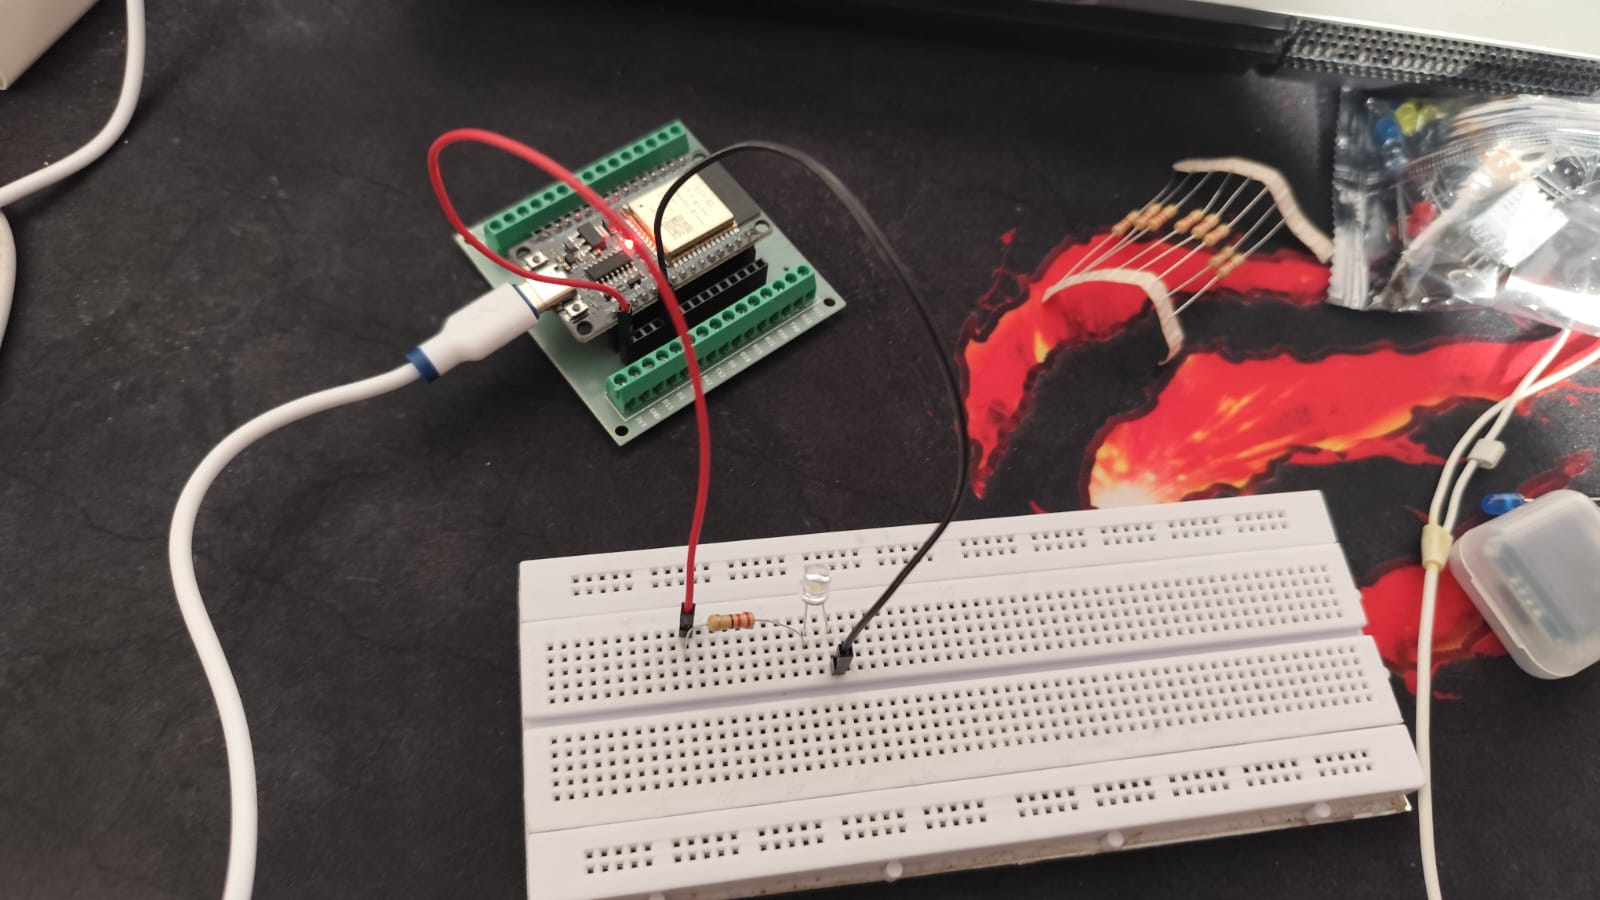
\includegraphics[width=\textwidth]{../Imagenes/On_Off_keyboard_imgs/On_Off_keyboard_img4.jpeg}
        \caption{Circuito con LED apagado}
        \label{fig:led_off}
    \end{subfigure}
    \caption{Montaje físico del proyecto On/Off Keyboard en protoboard}
    \label{fig:montaje}
\end{figure}

\begin{figure}[H]
    \centering
    \begin{subfigure}[b]{0.48\textwidth}
        \centering
        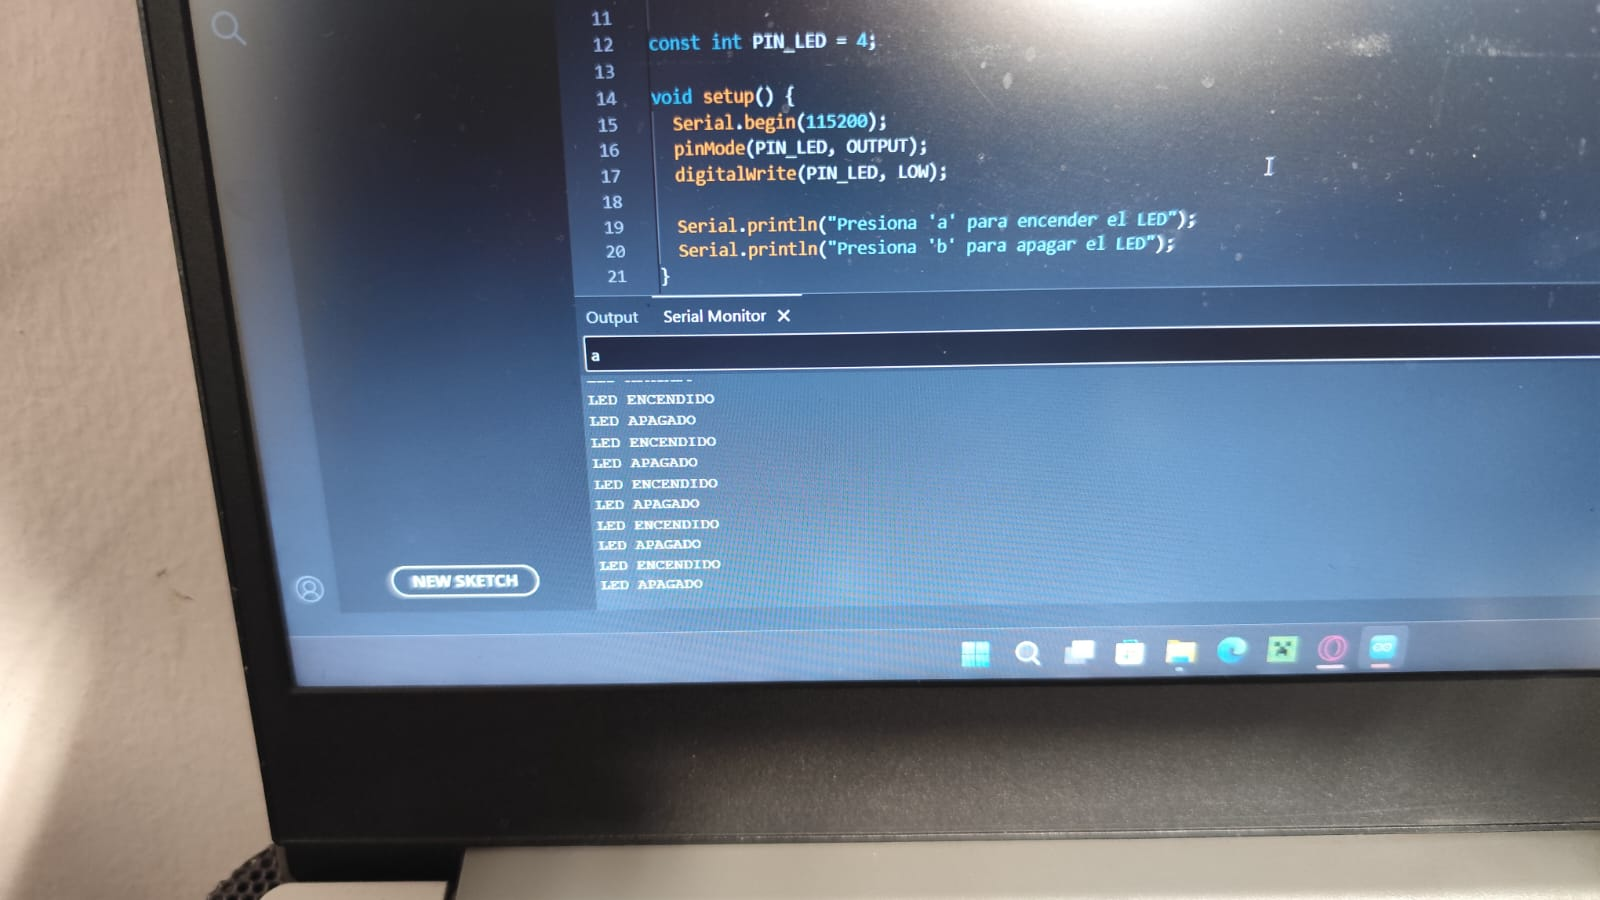
\includegraphics[width=\textwidth]{../Imagenes/On_Off_keyboard_imgs/On_Off_keyboard_img3.jpeg}
        \caption{Monitor Serial: enviando comando \texttt{a} para encender}
        \label{fig:serial_a}
    \end{subfigure}
    \hfill
    \begin{subfigure}[b]{0.48\textwidth}
        \centering
        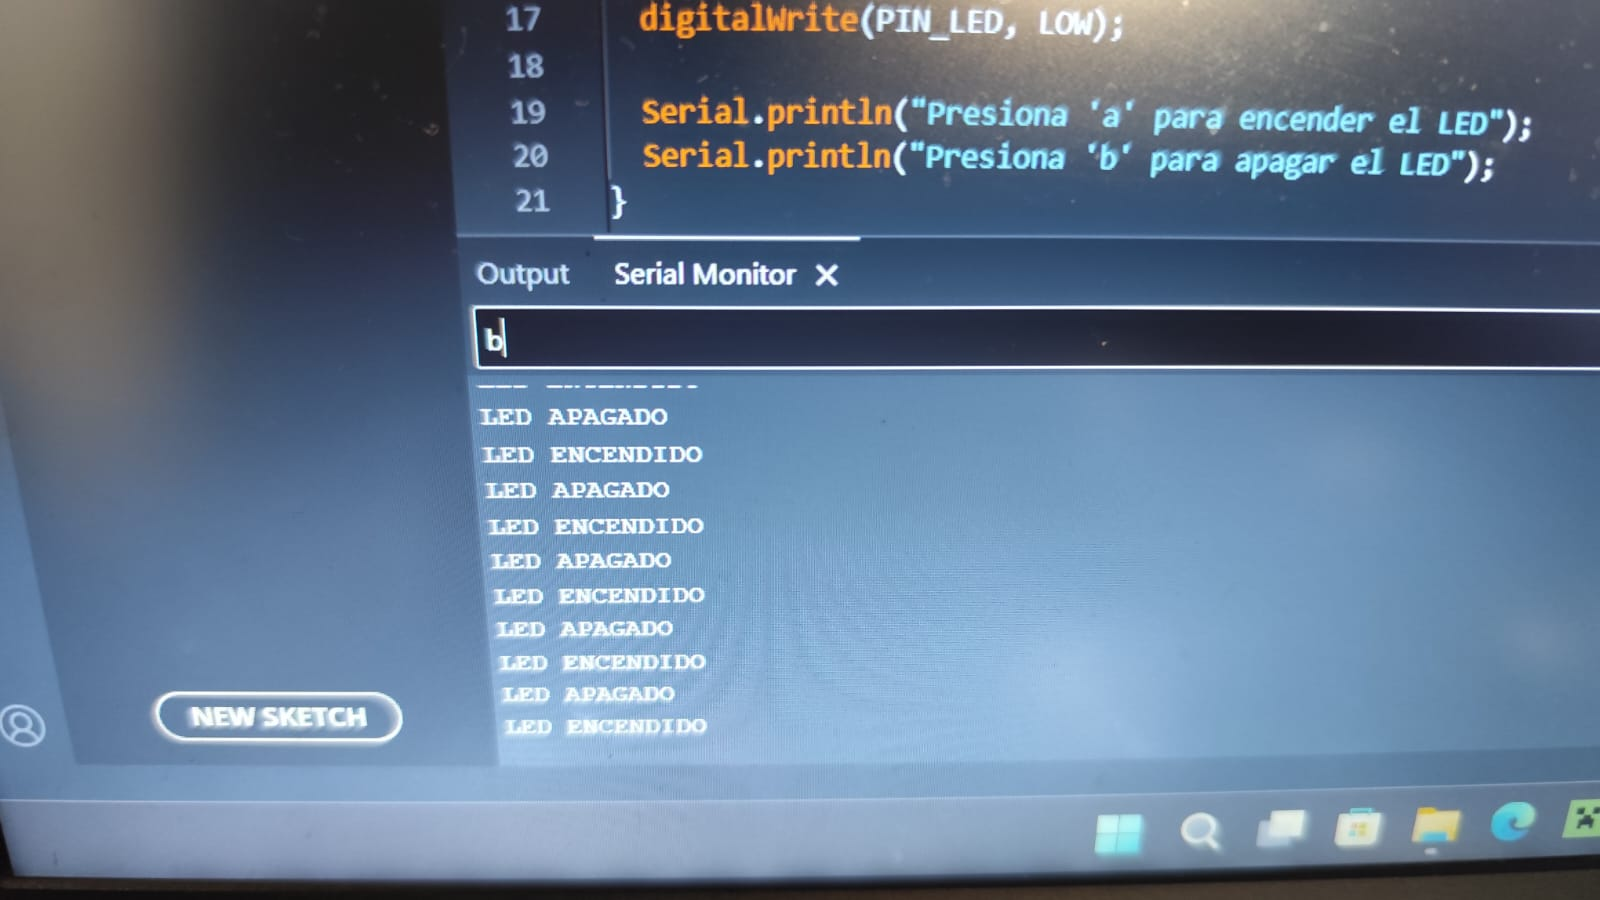
\includegraphics[width=\textwidth]{../Imagenes/On_Off_keyboard_imgs/On_Off_keyboard_img1.jpeg}
        \caption{Monitor Serial: enviando comando \texttt{b} para apagar}
        \label{fig:serial_b}
    \end{subfigure}
    \caption{Capturas del Monitor Serial mostrando la interacción con el programa}
    \label{fig:serial}
\end{figure}

En la Figura~\ref{fig:montaje} se observa el ESP32 conectado mediante USB al computador, con el LED y la resistencia montados en la protoboard. En la Figura~\ref{fig:serial} se aprecian las capturas del Monitor Serial del Arduino IDE, donde se alternan los mensajes ``LED ENCENDIDO'' y ``LED APAGADO'' según los comandos enviados por el usuario.

% ══════════════════════════════════════════════════════════════
\section{Video de Funcionamiento}
% ══════════════════════════════════════════════════════════════

El proyecto incluye un video demostrativo (\texttt{On\_Off\_Keyboard\_Funcionamiento.mp4}) que muestra el circuito en operación. En el video se puede observar cómo el usuario envía los caracteres \texttt{a} y \texttt{b} desde el Monitor Serial, y el LED responde encendiéndose y apagándose de forma inmediata, confirmando el correcto funcionamiento del código y las conexiones del circuito.

\textit{Nota: El archivo de video se encuentra en la carpeta \texttt{Videos/On\_Off\_Keyboard\_vid/} del proyecto.}

% ══════════════════════════════════════════════════════════════
\section{Proceso de Creación}
% ══════════════════════════════════════════════════════════════

El desarrollo de este proyecto siguió los siguientes pasos:

\begin{enumerate}
    \item \textbf{Diseño del circuito:} Se reutilizó el esquema del proyecto ``On/Off Repetitivo'' (LED + resistencia en GPIO4), ya que el hardware requerido es idéntico. El esquema fue diseñado en Fritzing.
    
    \item \textbf{Montaje en protoboard:} Se conectó el LED al pin D4 del ESP32 con una resistencia de 220\,$\Omega$ en serie, siguiendo el esquema de la Figura~\ref{fig:esquema}.
    
    \item \textbf{Desarrollo del firmware:} Se escribió el código en el Arduino IDE, incorporando:
    \begin{itemize}
        \item Lectura del buffer serial con \texttt{Serial.available()} y \texttt{Serial.read()}.
        \item Estructura condicional para interpretar los comandos \texttt{a}/\texttt{A} y \texttt{b}/\texttt{B}.
        \item Retroalimentación al usuario mediante mensajes en el Monitor Serial.
    \end{itemize}
    
    \item \textbf{Configuración del Arduino IDE:}
    \begin{itemize}
        \item Placa seleccionada: \textit{ESP32 Dev Module}.
        \item Velocidad de subida: 115200 baudios.
        \item Puerto: COM correspondiente al ESP32 conectado.
    \end{itemize}
    
    \item \textbf{Carga y prueba:} Se compiló y cargó el programa en el ESP32. Se abrió el Monitor Serial a 115200 baudios y se verificó el funcionamiento enviando los caracteres \texttt{a} y \texttt{b} repetidamente.
    
    \item \textbf{Documentación:} Se capturaron fotografías del montaje, capturas de pantalla del Monitor Serial, y se grabó un video demostrativo del funcionamiento.
\end{enumerate}

% ══════════════════════════════════════════════════════════════
\section{Conclusiones}
% ══════════════════════════════════════════════════════════════

\begin{itemize}
    \item El proyecto demuestra cómo utilizar la comunicación serial bidireccional para crear una interfaz de control básica entre el usuario y el microcontrolador.
    \item La función \texttt{Serial.available()} permite implementar un modelo de programación basado en eventos, evitando el uso de \texttt{delay()} que bloquea la ejecución del programa.
    \item La lectura de caracteres con \texttt{Serial.read()} y su evaluación con estructuras condicionales es el fundamento de protocolos de comunicación más complejos.
    \item El circuito físico (hardware) es idéntico al del proyecto ``On/Off Repetitivo'', lo que demuestra que un mismo montaje puede tener comportamientos completamente diferentes según el software que lo controle.
    \item La aceptación de mayúsculas y minúsculas mejora la experiencia del usuario y es una buena práctica de programación defensiva.
    \item Este proyecto constituye la base para sistemas de control más avanzados como: menús interactivos por consola, control de múltiples actuadores, y comunicación con aplicaciones externas vía serial.
\end{itemize}

\end{document}
